\cotefile{10}
\scanpage{115}
% archive sheet number: 114

Chapitre 1. Généralités sur les opérations $\otimes$ sur une catégorie.

\inserted{\handwritten{Appendice: Rappels sur les coalgèbres, comodules, bigèbres.....}}

Chapitre 2. Relations entre $\otimes$-catégories \deleted{et} avec foncteur fibre, et coalgèbres resp. hyperalgèbres: \deleted{\unsure{Group}} Dualité de Tannaka.

\hfill (structures mixtes, connexions ....)

Chapitre 3. \uline{Exemples nombreux et divers.} \uline{Dictionnaire détaillé.}

\margin{\handwritten{\figure{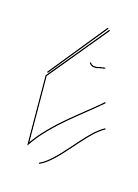
\begin{tikzpicture}[x=0.35cm,y=0.35cm]
\draw (2.9,4.8) -- (0.7,3.2);
\draw (2.95,4.72) -- (0.65,3.08) -- (0,0.6) .. controls (0.8,1.3) and (2,1.7) .. (2.8,2.1);
\draw (2.25,3.55) .. controls (2.35,3.3) and (2.55,3.4) .. (2.8,3.35);
\draw (0.4,-0.1) .. controls (1.1,0) and (2.1,1.0) .. (2.8,1.15);
\end{tikzpicture}}}}
Chapitre 4. Filtrations sur un foncteur fibre.

Chapitre 5. Théorème de structure des $\otimes$-catégories en termes de gerbes.

Chapitre 6. Polarisation d'une $\otimes$-catégorie. Groupes de Hodge.

Chapitre 7. $\otimes$-Catégories à lien réductif. Classification sur \uline{$R$}.

\unsure{8hapitre|Chapitre} 8. Structures de Hodge, groupes de Mumford-Tate et espaces modulaires correspondants.

Chapitre 9. Questions d'effectivité (?)

\handwritten{Éventuellement un chapitre de \unsure{Armature} sur le ``cas non commutatif''}

\handwritten{Un autre sur variantes pour catégories \uline{triangulées} ?}

\handwritten{Chapitre sur catégories de Picard,(plus gén.\ \unsure{gr.poïdes|g.poïdes} avec loi $\otimes$) catégories de Picard enveloppantes. Cas des catégories ayant deux loi $\oplus$ et $\otimes$ ----}

\scanpage{116}
% archive sheet number: 115

\uline{Chapitre} 1\qquad Généralités sur les $\otimes$-catégories.

\margin{\handwritten{\deleted{\unsure{catégories} \illegible{1} \unsure{exemples}}\par
\textcircled{1} produit tens. de modules\par
\textcircled{2} catégorie avec produits cart.\par
\textcircled{3} \unsure{torseurs} sous faisceau abélien\par
\textcircled{4} familles de \unsure{modules} \unsure{indexés} par \unsure{groupe}\par
\textcircled{5} espace des lacets d'un espace \fbox{topologique}}}

\uline{Par}.0: Lois $\otimes$ sur une catégorie: exemples divers ....

\uline{Par}.1 \deleted{Les données} Contraintes pour une loi $\otimes$ .

1.1. Associativité.

1.2. Commutativité.

1.3. Unités.

1.4. $\underline{\mathrm{Hom}}(X,Y),\ \underline{\mathrm{Moh}}(Y,X)$\handwritten{;} \handwritten{\deleted{$\unsure{X^\vee}$}} .

\inserted{\handwritten{\figure{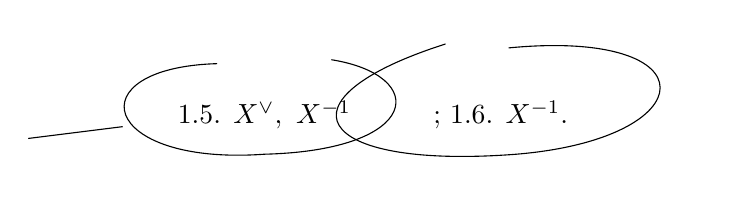
\begin{tikzpicture}[x=1cm,y=1cm]
\node at (0,0) {1.5. $X^\vee,\ \unsure{X^{-1}}$};
\node at (3,0) {; \deleted{\unsure{1.6.}} $X^{-1}$.};
\draw (-3,-.3) -- (-1.8,-.15);
\draw (-.6,.65) .. controls (-2.4,.6) and (-2.1,-.65) .. (0,-.5) .. controls (2,-.45) and (2.1,.5) .. (.85,.7);
\draw (2.3,.9) .. controls (.1,.2) and (.6,-.7) .. (3.2,-.5) .. controls (5.6,-.3) and (5.7,1.1) .. (3.1,.85);
\end{tikzpicture}}}}

\inserted{\handwritten{1.6. Cas des exemples du Par.0}}

\uline{Par}.2\qquad Compatibilités entre contraintes. \handwritten{(Toutes les \inserted{compatibilités entre} contraintes sont satisfaites, quand elles ont un sens, dans les exemples du par.0)}

1.1. Associativité et commutativité.

1.2. Commutativité et unité.

1.3. Associativité et unité.

1.4. \uline{Hom}, \uline{Moh} et associativité: formules de Cartan.

1.5. \uline{Hom} et commutativité (on a alors $\underline{\mathrm{Hom}}\inserted{\handwritten{(X,Y)}}\handwritten{\simeq}\underline{\mathrm{Moh}}\handwritten{(Y,X)}$\handwritten{)}.\handwritten{---}

\inserted{\handwritten{\deleted{(Lois $\otimes$ rigides)}}}

1.6. \uline{Hom} et unité : définition de $X^{\handwritten{\vee}}$ (pour loi commutative seulement ?).\margin{\figure{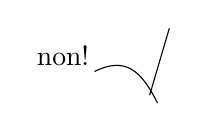
\begin{tikzpicture}[baseline]\node at (0,.4) {\handwritten{\uline{non!}}};\draw (.4,.2) .. controls (.8,.4) and (1,.2) .. (1.2,-.2);\draw (1.1,-.1)--(1.35,.75);\end{tikzpicture}}}

1.7. \inserted{\handwritten{\uline{Lois $\otimes$ rigides.}}} \handwritten{(}Formalisme des traces (cas \deleted{\illegible{1}} d'isomorphie $X^{\handwritten{\vee}}\otimes Y\handwritten{\simeq}\underline{\mathrm{Hom}}(X,Y)$).\handwritten{; rang d'un objet.}

\inserted{\handwritten{\uline{Par}.3}} \deleted{1.8.} Formes normales de multifoncteurs composés. \handwritten{\deleted{(\unsure{après le|pour le} \unsure{§} \uuline{\unsure{suivant}})}}

\uline{Par} \deleted{3}\handwritten{4}.\qquad $\otimes$-foncteurs.

\deleted{3}\handwritten{4}.1. Théorie sans contraintes: définition des $\otimes$-foncteurs, composition, morphismes de $\otimes$-foncteurs.

\deleted{3}\handwritten{4}.2. Compatibilité d'un $\otimes$-foncteur avec des contraintes: associativité et commutativité\handwritten{!}

\deleted{3}\handwritten{4}.3. Compatibilité avec des contraintes: unité.

\deleted{3}\handwritten{4}.4. Compatibilité avec des contraintes: \uline{Hom}, \uline{Moh}, \handwritten{$X^\vee,X^{-1}$ ---}

\inserted{\handwritten{4.5. Objets quasi-inversibles, et \deleted{\unsure{agrandissement} de \unsure{catégories}} \inserted{calcul} des fractions....}}

\uline{Par}. \unsure{4|5}.\qquad \uline{Exemples typiques:}\deleted{\illegible{1}} $\otimes$-\uline{catégories}\handwritten{\uline{définies par des bigèbres}.}

\inserted{\handwritten{5.0. $\otimes$-Catégories: (catégories additives, avec $\otimes$ biadditif, ass. comm. unit. \deleted{\unsure{avec}} \unsure{Gros} méc.\ \uline{$\unsure{\mathrm{Huy}|\mathrm{Hom}}$}).}}

\deleted{4}\handwritten{5}.1. Modules sur une bigèbre.

\deleted{4}\handwritten{5}.2. Comodules sur une bigèbre.

\deleted{4}\handwritten{5}.3. Dualité entre les deux notions: première manière (imparfaite).

\deleted{4}\handwritten{5}.4. Dualité entre les deux notions: seconde manière, formelle (via \deleted{\unsure{notions}} notions d'algèbre dans une $\otimes$-catégorie ).

\inserted{\handwritten{5.5. Modules mixtes (co + ordinaire) sur une bigèbre}}

\scanpage{117}
% archive sheet number: 116

\deleted{4}\handwritten{5}.6. Variantes avec bi-proalgèbres .

\deleted{4}\handwritten{5}.7. Variantes graduées.

\uline{Par}.\deleted{5}\handwritten{6} . Bigèbres d'endomorphismes des $\otimes$-foncteurs. Schémas en groupes d'automorphismes de $\otimes$-foncteurs.

....

\uline{Par} \deleted{6}\handwritten{7}. Structure des catégories de Picard\handwritten{(?)}(\unsure{Vinndrait|Viendrait} mieux avant par.4).

\margin{\handwritten{N'est pas \unsure{necessairement|nécessairement} le lieu ici}}

\handwritten{\deleted{\uline{Par}.8 \unsure{É|et}} Plus gén, \deleted{\unsure{catégories}}\inserted{\unsure{monoïdes|Monoïdes}} avec $\otimes$ associatif et unitaire (pas néc. comm. ...).}

\margin{\handwritten{\unsure{resp. com.}}}

\scanpage{118}
% archive sheet number: 117

$\otimes$-\uline{catégories}.

1) Définition. Catégorie \deleted{additiv} additive, avec bifoncteur
\[
(X,Y)\handwritten{\mapsto}X\otimes Y
\]
\deleted{et} un \deleted{objet} isomorphisme de bifoncteurs
\[
\handwritten{\phi}(X,Y,Z): (X\otimes Y)\otimes Z\handwritten{\xrightarrow{\sim}}X\otimes(Y\otimes Z)
\]
et un isomorphisme de commutativité
\[
\handwritten{\unsure{\mu|\psi}}(X,Y): X\otimes Y\handwritten{\xrightarrow{\sim}}Y\otimes X
\]
satisfaisant des axiomes

a) Axiome du pentagone pour $\handwritten{\phi}$ \deleted{(ne dépend pas de la structure additive)}

b) $\handwritten{\mu}(X,Y)\handwritten{\mu}(Y,X)=\mathrm{id}_{X\otimes X}$ \handwritten{;}

c) compatibilité entre $\handwritten{\phi}$ et $\handwritten{\mu}$ \handwritten{: axiome de l'hexagone}

d) existence d'un élément $1_C=\underline{1}$ , avec des isomorphismes fonctoriels
\[
u(X):\deleted{\unsure{x}}\quad\underline{1}\otimes X\handwritten{\simeq}X
\qquad\text{d'où}\quad
\inserted{v(X)=}\handwritten{\mu}(X,1)u(X): X\otimes1\handwritten{\simeq}X\ ,
\]
\figure{\handwritten{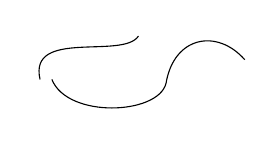
\begin{tikzpicture}[x=1cm,y=1cm]
\draw (-.75,.05) .. controls (-.9,.7) and (.3,.3) .. (.5,.6);
\draw (-.6,.05) .. controls (-.4,-.45) and (.75,-.4) .. (.85,0) .. controls (.95,.6) and (1.5,.7) .. (1.85,.3);
\end{tikzpicture}}}
% The preceding figure records the transposition/enclosure strokes on the two factors; the typed order is retained in the display.
(donc par b on aura aussi $u(X)=v(X)\handwritten{\mu}(1,X)$)

avec la condition que pour $X=\underline{1}$, on trouve le même isomorphisme
\[
u(\underline{1})=v(\underline{1}) :\qquad \underline{1}\otimes\underline{1}\handwritten{\simeq}\underline{1}
\]
ce qui s'exprime aussi par la condition que $\handwritten{\mu}(\underline{1},\underline{1})=\mathrm{id}_{\underline{1}}$ \handwritten{;}

\margin{\handwritten{\figure{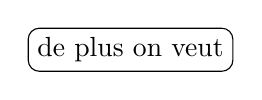
\begin{tikzpicture}
\node[draw,rounded corners,align=left] {de plus on veut};
\end{tikzpicture}}}}
\inserted{\handwritten{Compatibilité de $(\underline{1},u,v)$ avec $\unsure{\varphi|\phi}$, quand $X,Y$ \unsure{ou} $Z$ est \unsure{égal|ég.} à $1$, avec $\unsure{\psi|\mu}$ quand $X$ \unsure{ou} $Y$ est $=1$.}}

e) le foncteur $\otimes$ est biadditif.

\margin{\handwritten{\figure{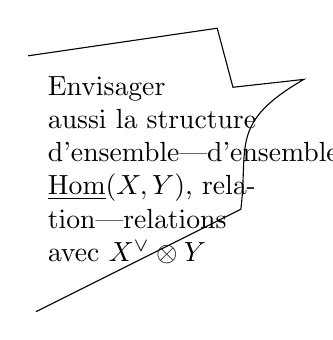
\begin{tikzpicture}[x=1cm,y=1cm]
\node[align=left,text width=2.7cm] at (0,0) {Envisager aussi la structure \unsure{d'ensemble|d'ensembles} $\underline{\mathrm{Hom}}(X,Y)$, \unsure{relation|relations} avec $X^\vee\otimes Y$};
\draw (-1.6,1.45) -- (.8,1.8) -- (1,1.05) -- (1.9,1.15) .. controls (.95,.6) and (1.2,.3) .. (1.1,-.5) -- (-1.5,-1.8);
\end{tikzpicture}}}}

NB a) \deleted{et d) sont}\inserted{est} indépendant\deleted{s} de la donnée de $\handwritten{\mu}$ , b) est indépendant de la donné de $\handwritten{\phi}$ , a)b)c)d) sont indépendant de fait que $C$ est additiv\deleted{\unsure{t}}e.

Soit $\underline{1}',u',\inserted{v'}$ comme $\underline{1},u,v$ , on va \deleted{définir canoniquement un}\inserted{\handwritten{voir qu'il existe un unique}} isomorphisme $w:\underline{1}\handwritten{\simeq}\underline{1}'$ , compatible en un sens évident avec $u,v$ et $u',v'$.

On choisit le composé
\diagram{\begin{tikzcd}[ampersand replacement=\&]
\underline{1} \arrow[r,"{\handwritten{\unsure{v'(1)|v(1)}}}"] \&
\underline{1}\otimes\underline{1}' \arrow[r,"{\handwritten{\unsure{u(\underline{1}')|\underline{1}\otimes u'}}}"] \&
\underline{1}'\deleted{\otimes\unsure{\underline{1}}} \arrow[r,phantom,"{\deleted{\longrightarrow}}" description] \& \deleted{\unsure{\underline{1}'}}
\end{tikzcd}}
. A vérifier les compatibilités annoncées (ne dépend pas de la donnée de $\handwritten{\phi}$, \inserted{ni $\handwritten{\mu}$,} mais de $u,v$ satisfaisant la compatibilité $\underline{u}(\underline{1})=v(\underline{1})$\deleted{\unsure{,}} et $u',v'$ kif-kif). C'est pourquoi il n'y\inserted{a} pas lieu de poser $\underline{1},u,v$ comme donnée, mais comme axiome d'existence.

\scanpage{119}
% archive sheet number: 118

2) $\otimes$-Foncteur $F:C\handwritten{\longrightarrow}C'$ (avec $C,C'$ des trucs-catégories).

Les données sont un foncteur \deleted{add} $F$, plus \deleted{\unsure{deu|deux}}un isomorphisme\deleted{s} de \unsure{bifoncteurs|bifoncteur}
\[
c(X,Y):F(X\otimes Y)\handwritten{\xrightarrow{\sim}}F(X)\otimes F(Y)
\]
\deleted{et isom.}
\[
\deleted{i:F(\underline{1}_C)\unsure{\longrightarrow|\simeq}\unsure{\underline{1}_{C'}|\underline{1}'_C}}
\]
satisfaisant les conditions:

a) Compatibilité \inserted{de $c$} avec la donnée de $\handwritten{\phi,\phi'}$

b) Compatibilité \inserted{de $c$} avec la donnée de $\handwritten{\unsure{\mu|\psi},\mu'}$

c) \deleted{Compatibilité de $i$ \unsure{avec} et $c$}\inserted{Existe isom.\ \deleted{fonct} $i\handwritten{\unsure{:|(}}F(\underline{1})\handwritten{\simeq}\underline{1}'$ compatible avec $c$ et} avec les isomorphismes $u\inserted{u'}$ (ou ce \deleted{\unsure{qui}} qui revient au même, avec \inserted{$c$ et} $v,v'$).

NB Cet $i$ sera alors uniquement déterminé.

d) $F$ est additif.

3) Homomorphisme d'un $\otimes$-foncteur $F$ dans un autre $G$: c'est un homomorphisme de foncteurs $f:F\handwritten{\longrightarrow}G$ satisfaisant le\deleted{s} condition

a) compatibilité avec \deleted{$c$ et} $c_F,c_G$

\handwritten{\deleted{\unsure{(A)|(a)} \unsure{pour} \illegible{2}}}

\deleted{b)} \handwritten{\deleted{\unsure{(A)|(a)}}(}compatibilité avec $i_F,i_G$ (\deleted{c'}\handwritten{\unsure{ce n'|car}} est \deleted{peut-être}\inserted{\handwritten{\deleted{\unsure{sans doute}} sans doute \unsure{pas une|par un}}} conséquence formelle de a) - à regarder\deleted{)}\handwritten{; cf plus bas)}

\handwritten{4)} \uline{Remarque\handwritten{s}}\qquad A dissocier \inserted{\handwritten{ce qui précède}} en plusieurs aspects de la donnée d'un bifoncteur\handwritten{$\otimes$}:

a) Donnée d'associativité, soumise à l'axiome du pentagone. Un foncteur ``compatible avec $\otimes$\inserted{associat\deleted{t}if''} de $C$ dans $C'$ est un foncteur $+$ un $c$ , compatible avec la donnée de $\handwritten{\phi}$ .

b) Donnée d'unité bilatère $\underline{1},u,v$ (unique à isomorphisme unique près). Un foncteur ``compatible avec \inserted{\handwritten{$\otimes$ à}} unité\deleted{s} bilatère\deleted{s}'' est un $F$ muni de $c$, tel qu'il existe $i$ compatible avec $c,u,v$ et $c',u',v'$ (lequel $i$ sera alors unique).

\margin{\handwritten{\uline{NB} Le monoïde des endom. de $\underline{1}$ est alors comm.}}

\handwritten{c)} Donnée de commutativité $\handwritten{\mu}$ , satisfaisant la condition de réflexivité.\deleted{(} Un foncteur

\scanpage{120}
% archive sheet number: 119

``compatible avec $\otimes$ èommutatif'' est un foncteur et un $c$, compatible avec la donnée des$\unsure{\otimes|\deleted{x}}$ $\handwritten{\unsure{\mu|\psi}}$ .

Quand on a une loi $\otimes$ avec donnée a) et b), il y a lieu de postuler une compatibilité entre les deux (dans le cadre del'axiomatique 1), est-ce une conséquence des autres axiomes ? je \deleted{crains}\inserted{\handwritten{pense}} que non, et qu'il faille le rajouter). Quand on a une loi $\otimes$ avec donnée a) et \unsure{v|c}), il y a lieu de postuler une compatibilité entre les deux. De même pour une loi $\otimes$ avec b) et c). Quand on a à la fois a)b)c), le paquet \deleted{\unsure{d'ax}} de toutes les conditions de compatibilité sont celles énoncées plus haut \inserted{dans 1º} a) à d) . De même, un Foncteur``compatible avec $\otimes$ associatif à \unsure{unité|mité} bilatère'' est un foncteur $F$, $+$ un $c$, compatible séparément avec associativité et unité bilatèrité, et de même pour tout autre paquet de données supplémentaires parmi a),b),c). Enfin, la notion d'homomorphisme de \deleted{\unsure{foncteu}} $\otimes$-foncteurs ne dépend pas des structures supplémentaires a)\deleted{b)} ou c) qu'on peut envisager\inserted{\handwritten{(mais bien de b)}} , s'exprimant exclusivement à l'aide de la donnée de $c$\deleted{\unsure{)}} \deleted{(sous réserve de vérification indiquée dans 3º)}. - Quan\deleted{d}\handwritten{t} a la \deleted{structure bilinéaire, il y a lieu de}\inserted{\deleted{\unsure{biaddiv|biadditiv}}} condition d'additivité sur les catégories et de biadditivité sur $\otimes$, il n'y a lieu de l'introduire qu'en dernier lieu.

\margin{Attention si l'associativité ne doit pas rappliquer ici aussi}
\deleted{5)}\inserted{\handwritten{5)}} NB Si on a $\otimes$ avec unité bilatère, alors pour deux endomorphismes $u,v$ de $\underline{1}$, on a $u\otimes v\overset{\handwritten{!}}{=}uv=vu$. Donc sous la condition de commutativité\deleted{\unsure{x|,}} c), $\unsure{\mathbb{E}|\mathrm{E}}\mathrm{nd}(\underline{1})$ est un monoïde commutatif. \inserted{\deleted{il opère sur tous}}\deleted{Si $\underline{C}$ est additif, c'est} Sans condition de comm. ce monoïde opère à gauche et à droite sur tout objet de $\underline{C}$; les deux opérations coïncident moyennant commutativité. Si \deleted{la structure}\inserted{$C$} est add\unsure{i|o}tive, $\mathrm{End}(\underline{1})$ est un anneau, qui opère à gauche et à droite sur chaque objet de $C$. Dans le cas commutatif, $\mathrm{End}(\underline{1})=\unsure{\mathbb{k}|k}$ est donc un anneau commytatif et la catégorie $C$ est $k$-linéaire de façon naturelle\handwritten{, $\otimes$ est $k$-bilinéaire.}

\scanpage{121}
% archive sheet number: 120

6) Supposons maintenant que $C$ soit une catégorie \deleted{additive}\inserted{abélienne} $k$-linéaire ($k$ un corps) munie d'un foncteur fidèle exact $F:C\handwritten{\to}\mathrm{Modf}(k)$, de sorte que $C$ s'identifie à la catégorie des représentations \deleted{d'un}\inserted{(continues)} finies d'une algèbre profinie $U$ sur $k$\inserted{(associative, unitaire)}, ou des comodules sur le dual\inserted{topologique} $A$ de $k$, qui est une coalgèbre (associative, unitaire). Alors la donnée d'un foncteur $\otimes$\inserted{bilinaire} compatible avec $F$ (i.e. pour lequel \deleted{c'est} on a \uline{égalité} $F(X\otimes Y)=F(X)\otimes F(Y)$) \uline{équivaut} à la donnée d'un morphisme diagonal $U\handwritten{\to}U\overset{\handwritten{\scriptscriptstyle\wedge}}{\otimes}_k U$, ou encore d'une loi de multiplication sur $A$. Une donnée supplémentaire (au sens de 4)) a) \deleted{b)}\inserted{\handwritten{b)}} ou c) \uline{compatible} avec $F$, $c=\mathrm{id}$ est alors uniquement déterminée, si elle existe.\inserted{\handwritten{\deleted{\unsure{pour b)} \unsure{il} \illegible{4} \unsure{que soit une} $\unsure{\epsilon|\varepsilon}:U\to k$ (\unsure{hom. de $k$-alg}) i.e. $\epsilon\in A$ \unsure{et que ce soit}}}} Elle existe sss $A$ est associative, resp. unitaire resp. commutative. Quand ces conditions sont satisfaites simultanément, on a donc un schéma en \deleted{groupes}\inserted{\handwritten{monoïdes}} affine sur $k$, qui permet de réconstituer la situation. - Si on a de même $\mathbb{C}',F'$ sur le même $k$, \deleted{avec un $\otimes$,} alors les foncteurs $G:C\handwritten{\to} C'$ compatibles avec $F,F'$ correspondent exactement aux hom. de $k$-algèbre top $U'\handwritten{\to}U$, ou de $k$-coalgèbres $A\handwritten{\to}A'$. Si $\mathbb{C}$ et $C'$ sont munis de structures bilinéaires $\otimes\handwritten{\unsure{,|/}}\otimes$, alors le foncteur $G$ est un $\otimes$-foncteur avec un isomorphisme $c$ transformé par $F'$ en $\mathrm{id}$ (ce qui suffit à \deleted{le} caractériser\inserted{\handwritten{$c$}} alors) sss $U'\handwritten{\to}U$ est compatible avec les diagonales i.e. $A\handwritten{\to}A'$ est compatible avec les multiplications. Les éventuelles structures supplémentaires a) \deleted{b)} ou c) sont respectées automatiquement,\inserted{\handwritten{pour b) il faut imposer compatibilité aux \unsure{augm.|augm} de $U$ resp. aux unités de $A,A'$}}

\margin{généraliser au moins partiellement au cas d'un $k$ qui n'est pas un corps}

\margin{\figure{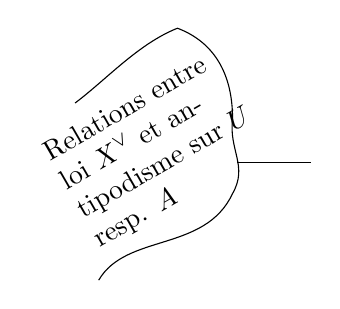
\begin{tikzpicture}[baseline]
\draw (0,0) .. controls (.35,.6) and (1.35,.35) .. (1.7,1.1) .. controls (1.9,1.45) and (1.65,1.65) .. (1.7,2.05) .. controls (1.7,2.7) and (1.4,3.05) .. (1,3.2) .. controls (.5,3) and (.1,2.55) .. (-.3,2.25);
\draw (1.76,1.5)--(2.7,1.5);
\node[rotate=30,align=left,text width=2.65cm] at (.8,1.7) {\handwritten{Relations entre\\loi $X^\vee$ et antipodisme sur $U$\\resp. $A$}};
\end{tikzpicture}}}

\figure{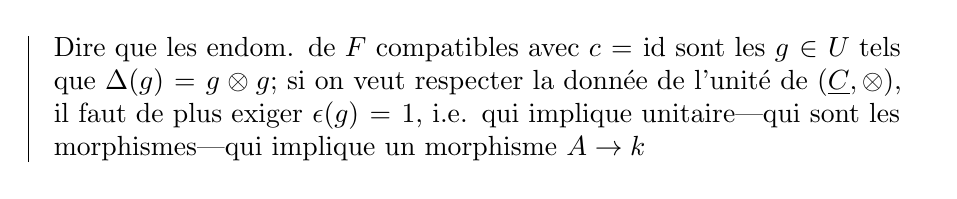
\begin{tikzpicture}[baseline]
\draw (0,0)--(0,1.6);
\node[anchor=west,align=left,text width=11cm] at (.2,.8) {\handwritten{Dire que les endom. de $F$ compatibles avec $c=\mathrm{id}$ sont les $g\in U$ tels que $\Delta(g)=g\otimes g$; si on veut respecter la donnée de l'unité de $(\underline{C},\otimes)$, il faut de plus exiger $\epsilon(g)=1$, i.e. \unsure{qui implique unitaire|qui sont les morphismes|qui implique un morphisme} $A\to k$}};
\end{tikzpicture}}

7) Un exemple. On prend pour $C$ la catégorie des modules gradué\unsure{ss|s} sur un anneau commutatif $\mathbb{k}$, avec le produit tensoriel gradué ordinaire et pour unité le module $\mathbb{k}_s$ gradué par le degré zéro, donnée\deleted{\unsure{di}} de $u$ et $v$ comme d'habitude, ainsi que $\handwritten{\phi}$ (associativité) et $\handwritten{\unsure{\mu|\psi}}$ (commutativité). Tous les axiomes du nº1 sont vérifiés, et le foncteur oubli (avec $c=\mathrm{id}$) estnun $\otimes$-foncteur respectant toutes les données a)b)c). Donc si $k$ est

\scanpage{122}
% archive sheet number: 121

corps et si on se borne aux modules de type fini sur $k$, on est dans les conditions de 6), et on trouve le groupe algébrique $\underline{G}_m$ sur $k$. D'ailleurs même sans condition sur $k$ et sans se borner à des modules de type fini, on récupère $C$ avec toutes ces structures par les représentations de $\underline{G}_m$\handwritten{\unsure{!|/|.}}

Gardons $\otimes$, $\handwritten{\phi}$ (et $\underline{1},u,v$) comme dessus, mais changeons $\handwritten{\unsure{\psi|\mu}}$ \deleted{ou $\handwritten{\unsure{\phi|\psi}}$}, en \deleted{\unsure{tri}} utilisant la règle de Koszul. Ce\inserted{\handwritten{nouveau}} choix de $\handwritten{\mu}$ s'impose dans certaines questions. Par exemple supposons $k$ un corps, \deleted{de car. nulle,} soit $V$ la catégorie des espaces topologiques compacts, avec le foncteur $\otimes$ donné \unsure{par} produit cartésien, et la donnée évidente d'associativité et de commutativité (pour le c\deleted{\unsure{a}}oup on n'a vraiment pas le choix !); il y a\deleted{\unsure{x}} une unité, \unsure{à} savoir l\deleted{\unsure{es}}'espace\deleted{s} ponctuel. Considérons le foncteur cohomologique $X\handwritten{\mapsto}H^{\handwritten{\bullet}}(X,k)$ sur $V^{\unsure{o|0}}$, utilisant Künneth on trouve un isomorphisme $c$ de compatibilité aux $\otimes$\inserted{de $V^o$ dans $C$}. Ce dernier est compatible aux structures a),b),c) \uline{à condition} de choisir $\handwritten{\mu}$ dans $C$ par la règle de Koko\deleted{\unsure{f}}!

A prouver que lorsque on prend $C$comme dessus à la Koko, il n'y\deleted{\unsure{a}} a pas de foncteur fibre sur $C$ sur aucune extension $K$ de $k$ (même en\deleted{\unsure{s}} se bornant aux vectoriels de dim\unsure{e|m}nsion finie) !

% Thin separation stroke between C and comme in the preceding paragraph.
\figure{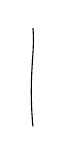
\begin{tikzpicture}[baseline]\draw (0,-.55) .. controls (-.06,.1) and (.03,.4) .. (0,.7);\end{tikzpicture}}

\margin{???}
\margin{\figure{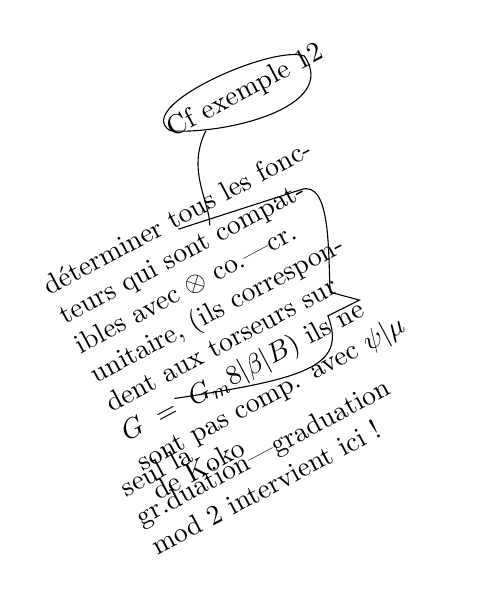
\begin{tikzpicture}[baseline]
\node[rotate=28] at (1.05,4.9) {\handwritten{Cf exemple 12}};
\draw (.1,4.4) .. controls (-.4,4.7) and (1.4,5.5) .. (1.8,5.35) .. controls (2.25,4.7) and (.8,4.35) .. (.1,4.4);
\draw (.55,4.4) .. controls (.3,3.9) and (.6,3.5) .. (.6,3.2);
\draw (.2,3.15)--(1.75,3.65) .. controls (2.15,3.8) and (2.1,2.8) .. (2.13,2.35)--(2.5,2.25)--(2.1,2.05) .. controls (2.35,1.4) and (1.8,1.25) .. (.15,1.0);
\node[rotate=28,align=left,text width=4.2cm] at (1.05,2.1) {\handwritten{déterminer tous les foncteurs qui sont compatibles avec $\otimes$ \unsure{co.|cr.} unitaire, \unsure{(}ils correspondent aux torseurs sur $G=G_m\unsure{8|\beta|B}$) \uline{ils ne sont pas comp. avec $\unsure{\psi|\mu}$ de Koko}}};
\node[rotate=28,align=left,text width=3.9cm] at (1.4,.4) {\handwritten{seul la \unsure{gr.duation|graduation} mod $2$ intervient ici !}};
\end{tikzpicture}}}

Pour pallier à cet inconvénient, il y a lieu\deleted{\unsure{lorsqu'on s'en va dans} une \unsure{catégori|catégorie} avec $\otimes$ la catégorie des} d\deleted{\unsure{e}}'étudier systématiquement les $\otimes$-foncteurs compatibles avec a)b)c) à valeurs dans une catégorie\inserted{de modules \unsure{grad|gradués}} $\mathbb{C}$ comme ci-dessus: ce sont \handwritten{l}es\handwritten{``}\uline{foncteurs fibres tordus}\handwritten{''}. En particulier, si $C$ est comme au début de 6) (pas encore de $\otimes$), supposons que le foncteur $F$ se factorise (de façon donnée) par les modules gradués, i.e. qu'on ait un foncteur compatible avec les foncteurs oublis $C\handwritten{\to}\mathrm{Gradf}(k)\unsure{=|\equiv}\mathbb{D}^{\unsure{\mathbb{X}|X}}$. Cela correspond à un homomorphisme de coalgèbres de $A$ dans $k\handwritten{[}T,T^{-1}\handwritten{]}$; où à la donnée d'éléments $\handwritten{\pi}_i$ de $U$ (les projections sur les composants homogènes) satisfaisant les conditions \deleted{$\unsure{\handwritten{\pi}_i=0_i|\handwritten{\pi}_i\pi_i=0}$} habituelles
